\documentclass[12pt]{article}
\usepackage[margin=1in]{geometry}
\usepackage{amsfonts, amsmath, amssymb}
\usepackage{hyperref}
\usepackage{mathtools}
\hypersetup{
    colorlinks=true,
    linkcolor=blue,
    filecolor=magenta,      
    urlcolor=cyan,
}
\usepackage{graphicx}
\usepackage{fancyhdr}
\setlength{\headheight}{15pt}

\pagestyle{fancy}
\fancyhf{}

\rhead{
  Shengdong Li
  Calc 3
}

\rfoot{
  Page \thepage
}

% \usepackage{indentfirst}

\begin{document}
\title{Initial D++}
\author{by Shengdong Li}
\date{16 October 2020}
\maketitle

\begin{align}
  \intertext{\textbf{D)} Motion and Physics: You have been asked to consult on the new Hollywood blockbuster called "Houston, We Have a Problem."  The plot line is that the main character (played by Scarlett Johansson) is working for NASA in a division that is monitoring the health of a very old geostationary satellite. 15 minutes into the movie, a small meteorite hits the satellite in such a way that it knocks the satellite out of orbit as well as taking out the thrusters built to stabilize the satellite at the end of its life. The satellite is in total free fall towards Houston.  Only Scarlett, and her love interest Mark Ruffalo, can save Houston now. Unfortunately, for you, the writers pretty much had no idea what they were doing when they created the plot, so they need you to help them get their math set.}
  \intertext{\textbf{Part 1} According to the script, when the satellite began its free fall, the satellite was \textbf{36,000 kilometers} with no downward velocity, but with a downward acceleration matching the gravitational constant of  \textbf{$9.8m/s^2$}.  Use this information to create \textbf{(a)} a differential for the change in velocity at a given time as well as the particular solution associated and \textbf{(b)} a differential for the height of the satellite at a given time as well as the particular solution associated.  With this information, at what velocity will the satellite be traveling when it obliterates Houston? }
  \intertext{The change in velocity at a given time can be modeled using the acceleration constant}
  \Aboxed{\frac{dv}{dt}   & =-9.8}                                                                         \\
  \intertext{Solve for general solution for velocity over time using separation of variables}
  \int_{ }^{ }dv          & =\int_{ }^{ }-9.8dt                                                            \\
  v                       & =-9.8t+C                                                                       \\
  \intertext{Solve for particular solution for velocity over time using (0,0)}
  0                       & =-9.8\left(0\right)+C                                                          \\
  C                       & =0                                                                             \\
  \Aboxed{v               & =-9.8t}                                                                        \\
  \intertext{The change in height of a satellite at a given time is just velocity}
  \frac{dh}{dt}           & =v                                                                             \\
  \Aboxed{\frac{dh}{dt}   & =-9.8t}                                                                        \\
  \intertext{Solve for general solution for height at a given time using separation of variables}
  \int_{ }^{ }dh          & =-9.8\int_{ }^{ }tdt                                                           \\
  h                       & =-4.9t^{2}+C                                                                   \\
  h                       & =-4.9t^{2}+C                                                                   \\
  \intertext{Solve for particular solution for height at a given time using (0, 36000000)}
  36000\ km\              & =\ 36000000\ m                                                                 \\
  36000000                & =-4.9\left(0\right)^{2}+C                                                      \\
  C                       & =36000000                                                                      \\
  \Aboxed{h               & =36000000-4.9t^{2}}                                                            \\
  \intertext{The question ``With this information, at what velocity will the satellite be travelling when it obliterates Houston?''}
  \intertext{Is basically asking: At height 0, what is the velocity?}
  \intertext{Solve for $t$ at $h=0$}
  0                       & =36000000-4.9t^{2}                                                             \\
  36000000                & =4.9t^{2}                                                                      \\
  t^{2}                   & =\frac{36000000}{4.9}                                                          \\
  t                       & =\left(\frac{36000000}{4.9}\right)^{\frac{1}{2}}                               \\
  t                       & =2710.52                                                                       \\
  \intertext{Plugin this t to the velocity over time function}
  v                       & =-9.8\left(\left(\frac{36000000}{4.9}\right)^{\frac{1}{2}}\right)              \\
  \Aboxed{v               & =-26563.13}                                                                    \\
  \intertext{\textbf{Ans.} -26563.13 $\frac{m}{s}$ is the velocity at which the satellite will be traveling when it crashes into Houston.}
  \intertext{\textbf{Part 2} According to the very loose research the writers did, wind resistance will end up slowing the satellite down starting at about \textbf{600 km} above Houston.  This wind resistance will cause the downward velocity to decrease at a rate proportional to the velocity.  Use the models above to determine the velocity at which the satellite will be travelling when it reaches 600 km above the earth and use this as your new initial value to determine the particular solution (in terms of the currently unknown proportionality constant, k ).   }
  \intertext{First find the $t$ at height 600 km using our height function earlier}
  600\ km\                & =600000\ m                                                                     \\
  h                       & =36000000-4.9t^{2}                                                             \\
  600000                  & =36000000-4.9t^{2}                                                             \\
  35400000                & =4.9t^{2}                                                                      \\
  t^{2}                   & =\frac{35400000}{4.9}                                                          \\
  t                       & =\left(\frac{35400000}{4.9}\right)^{\frac{1}{2}}                               \\
  t                       & =2687.84                                                                       \\
  \intertext{Then plug this time into our velocity function}
  v                       & =-9.8\left(\left(\frac{35400000}{4.9}\right)^{\frac{1}{2}}\right)              \\
  \Aboxed{v               & =-26340.84}                                                                    \\
  \intertext{\textbf{Ans.} The satellite will be travelling at $-26340.84\frac{m}{s}$ when it reaches $600\:km$ above earth.}
  \intertext{Now we setup our new velocity function: First the downward velocity increase would still be from gravity}
  -9.8                                                                                                     \\
  \intertext{However, the velocity decrease would be a proportion of the total velocity}
  kv                                                                                                       \\
  \intertext{We can put this all together in one function}
  \frac{dv}{dt}           & =-9.8+kv                                                                       \\
  \intertext{This can actually be rearranged into the standard form of an FOLE}
  v'                      & =-9.8+kv                                                                       \\
  v'-kv                   & =-9.8                                                                          \\
  \intertext{Solve for the general solution for velocity at a given time.}
  I\left(x\right)         & =e^{\int_{ }^{ }-kdt}                                                          \\
  I\left(x\right)         & =\frac{1}{e^{kt}}                                                              \\
  y                       & =\frac{1}{I\left(x\right)}\int_{ }^{ }I\left(x\right)P\left(x\right)dx         \\
  v                       & =-9.8e^{kt}\int_{ }^{ }\frac{1}{e^{kt}}dt                                      \\
  u                       & =-kt                                                                           \\
  -\frac{1}{k}du          & =dt                                                                            \\
  v                       & =\frac{1}{k}\cdot9.8e^{kt}\int_{ }^{ }e^{u}du                                  \\
  v                       & =\frac{1}{k}\cdot9.8e^{kt}\left(e^{-kt}+C\right)                               \\
  v                       & =\frac{9.8}{k}+Ce^{kt}                                                         \\
  v                       & =Ce^{kt}+\frac{9.8}{k}                                                         \\
  \intertext{Now we solve for the C (in terms of k) using the velocity at height $600\:km$ that we got earlier to get our particular solution}
  -26340.84               & =C+\frac{9.8}{k}                                                               \\
  -26340.84-\frac{9.8}{k} & =C                                                                             \\
  \intertext{\textbf{Ans.} The particular solution for velocity in terms of $k$ will be}
  \Aboxed{v               & =\left(-26340.84-\frac{9.8}{k}\right)e^{kt}+\frac{9.8}{k}}                     \\
  \intertext{\textbf{Part 3} The current script has around 15 minutes of plot building and around 15 minutes at the end of wrapping up the movie.  They want to have the remaining part of the movie be in "real time" and want you to tell them about the timeline.   This will allow them to figure out how to structure the sub-plots within the context of the impending disaster.  As part of this, they want Mark and Scarlett to declare their undying love  when the satellite hits the 600 km elevation, which will be the same time they turn on their giant fan to increase the wind resistance, slow down the satellite, and save Houston. To start, they want to know how long Mark and Scarlett would have, once the satellite is 600 km above the Earth, if there were no wind resistance.  Determine what the k would be with no wind resistance.  Then determine how long would they have from the moment the meteorite hit?  How long would they have once the satellite is 600 km above the Earth? }
  \intertext{If the wind resistance was 0, you could reason that v' would just equal the acceleration constant}
  v'                      & =-9.8+kv                                                                       \\
  -9.8                    & =-9.8+kv                                                                       \\
  \intertext{Now solve for k}
  0                       & =kv                                                                            \\
  \Aboxed{k               & =0}                                                                            \\
  \intertext{However, the above k value doesn't matter. To solve for the amount of time left at 600 km, we can just use our previous values for total time it takes for meteor to fall and time it took to get to 600 km, which we've already calculated}
  \Aboxed{2710.52-2687.84 & =22.68}                                                                        \\
  \intertext{\textbf{Ans.} From the point at which the meteor is 600 km up, they would have $22.68\:s$ until the meteor hit Houston.}
  \intertext{\textbf{Part 4} Their first idea is that the fan, combined with air resistance, would be powerful enough to stop the satellite from accelerating further, meaning that whatever velocity occurs when the satellite hits 600 kilometers above the earth is the velocity it will travel to the Earth's surface.  What would the k be in this case? If the satellite travels at this constant speed for the remaining 600 kilometers, how much time would Scarlett and Mark have to declare their undying love? }
  \intertext{This is basically asking what the k should be to keep the velocity the exact same (i.e. $-26340.84\frac{m}{s}$ at $h=600\:km$). To determine this, let's first set $f'=0$ and determine the equilibrium solution for our change in velocity}
  v'                      & =-9.8+kv                                                                       \\
  0                       & =-9.8+kv                                                                       \\
  9.8                     & =kv                                                                            \\
  \intertext{And so this is our equilibrium solution}
  \frac{9.8}{k}           & =v                                                                             \\
  \intertext{Now we can solve for k by plugging in the velocity that we want!}
  v                       & =-26340.84                                                                     \\
  -26340.84               & =\frac{9.8}{k}                                                                 \\
  k                       & =\frac{9.8}{-26340.84}                                                         \\
  \Aboxed{k               & =-0.000372045842122}                                                           \\
  \intertext{However, we don't actually need to use the k value to solve for time until impact, we can just use use the velocity function from part 1. }
  -26340.84t              & =-600000                                                                       \\
  t                       & =\frac{-600000}{-26340.84}                                                     \\
  \Aboxed{t               & =22.78}                                                                        \\
  \intertext{\textbf{Ans.} If the satellite travels at constant speed for the remaining 600km to Houston, there will be around $22.78\:s$ for Scarlett and Mark to declare their undying love.}
  \intertext{\textbf{Part 5} At this point, the writers are pretty upset that their plans for their plot are completely falling apart.  You're not sure if it will help or hurt, so you mention the idea of terminal velocity.  This is the concept that wind resistance slows things down proportional to their velocity, which means that at some point an object falling towards earth will stop accelerating and maintain a constant velocity.  The terminal velocity for the average sky diver is 54 meters per second, so this would be a good starting point for the satellite (though terminal velocity would be more complicated).  The writers decide to scrap their entire plot and re-write the movie so that Scarlett and Mark are now EMTs trying to save Houston from a container full of a toxin dropped at 600 kilometers above Houston.  Their job is to help evacuate the city.  Using the model from (2) and the knowledge that the initial velocity was 0 when the container was dropped at 600 kilometers, solve for the differential and particular solution with respect to k.  To find k, use your knowledge of equilibrium solutions.  Once you have k, solve for the height function to determine how long you have until the container reaches Earth.  }
  \intertext{Using the model from part 2, We can get the solution in terms of k if we plug in (0,0)}
  v                       & =Ce^{kt}+\frac{9.8}{k}                                                         \\
  0                       & =C+\frac{9.8}{k}                                                               \\
  C                       & =-\frac{9.8}{k}                                                                \\
  v                       & =-\frac{9.8}{k}e^{kt}+\frac{9.8}{k}                                            \\
  v                       & =\frac{9.8}{k}\left(1-e^{kt}\right)                                            \\
  \intertext{To get the value of k, we first have to look at current possible equilibrium solutions by setting f'=0}
  v'                      & =-9.8+kv                                                                       \\
  0                       & =-9.8+kv                                                                       \\
  9.8                     & =kv                                                                            \\
  v                       & =\frac{9.8}{k}                                                                 \\
  \intertext{This means that the value of v is stable when $\frac{9.8}{k}$ is v. Therefore if we want v to stabilize at -54 we can just plugin -54 and solve for k}
  -54                     & =\frac{9.8}{k}                                                                 \\
  -54k                    & =9.8                                                                           \\
  \Aboxed{k               & =-\frac{9.8}{54}}                                                              \\
  \intertext{And to check that our velocity will approach -54, we can plugin k}
  v                       & =\frac{9.8}{\left(-\frac{9.8}{54}\right)}                                      \\
  v                       & =-54                                                                           \\
  \intertext{Now plugging in this k gives us the full velocity function of}
  v                       & =-54\left(1-e^{-\frac{9.8}{54}t}\right)                                        \\
  v                       & =54\left(e^{-\frac{9.8}{54}t}-1\right)                                         \\
  \intertext{Now we can setup the height differential equation, which again, is just velocity}
  \frac{dh}{dt}           & =54\left(e^{-\frac{9.8}{54}t}-1\right)                                         \\
  \intertext{Solve it for the general solution of height}
  \int_{ }^{ }dh          & =54\int_{ }^{ }e^{-\frac{9.8}{54}t}-1dt                                        \\
  h                       & =54\left(\int_{ }^{ }e^{-\frac{9.8}{54}t}dt-\int_{ }^{ }dt\right)              \\
  u                       & =-\frac{9.8}{54}t                                                              \\
  du                      & =-\frac{9.8}{54}dt                                                             \\
  -\frac{54}{9.8}du       & =dt                                                                            \\
  h                       & =54\left(-\frac{54}{9.8}\int_{ }^{ }e^{u}dt-t\right)                           \\
  h                       & =54\left(-\frac{54}{9.8}e^{-\frac{9.8}{54}t}-t\right)                          \\
  h                       & =-\frac{\frac{2916}{9.8}}{e^{\frac{9.8}{54}t}}-54t+C                           \\
  \intertext{Now solve for the specific solution knowing that the drop starts at 600km}
  600\ km\                & =\ 600000\ m                                                                   \\
  600000                  & =-\frac{\frac{2916}{9.8}}{e^{\frac{9.8}{54}\left(0\right)}}-54\left(0\right)+C \\
  600000                  & =-\frac{2916}{9.8}+C                                                           \\
  C                       & =600000+\frac{2916}{9.8}                                                       \\
  C                       & =\frac{5882916}{9.8}                                                           \\
  \Aboxed{h               & =-\frac{\frac{2916}{9.8}}{e^{\frac{9.8}{54}t}}-54t+\frac{5882916}{9.8}}
\end{align}
The only way that I really know how to solve this h is by graphing it...
\begin{figure}[ht]
  \begin{center}
    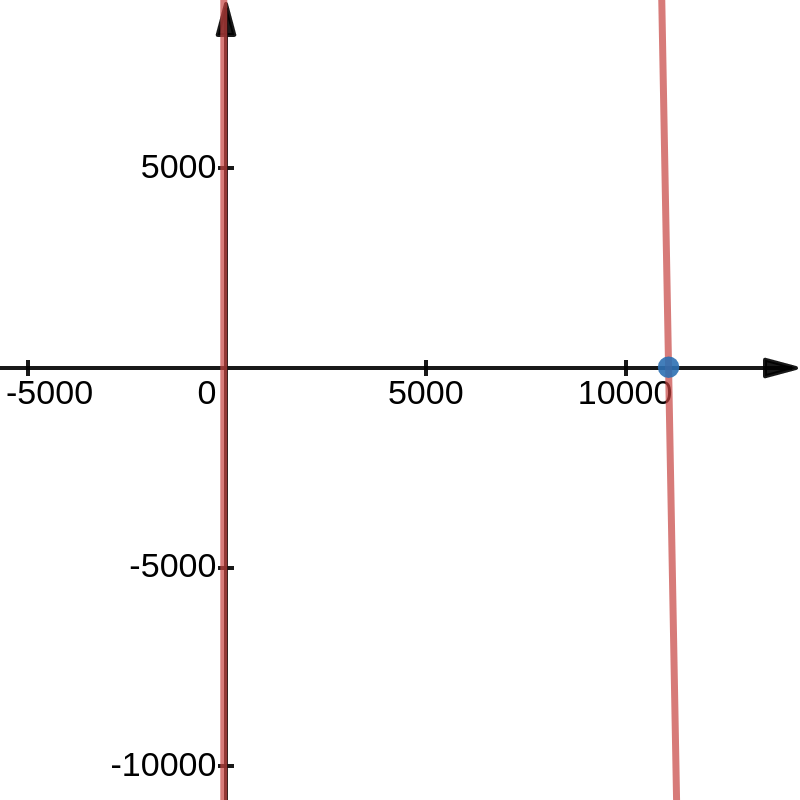
\includegraphics[scale=.3]{disc-5-terminal-velocity-height-function.png}
    \caption{\textit{Graph of the height function.} Desmos link \href{https://www.desmos.com/calculator/cvnkkwav9r}{\textcolor{blue}{here}}}
  \end{center}
\end{figure}
\begin{align}
  \intertext{...then looking at where the x intercepts are. One happens to be at }
  t         & =11116.62  \\
  \intertext{and another at }
  t         & =-41.95    \\
  \intertext{But since it doesn't make any sense for $t$ to be negative, we choose the positive variant}
  \Aboxed{t & =11116.62}
\end{align}
\textbf{Ans.} There are about $11116.62\: s$ until the container full of toxin drops on Houston.
\end{document}